\documentclass[10pt]{article}
\usepackage{ctex}
\usepackage{CJK}
\usepackage{graphicx}
\usepackage{graphicx}
\bibliographystyle{plain}
\setlength{\parindent}{2em}
\begin{document}
\title{5G mobile phone}
\author{Qilei Zhang}
\date{may 15 2018}
\maketitle
\par
\begin{figure}[htbp]
\small
\centering
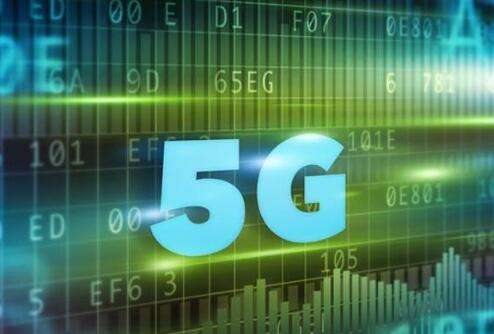
\includegraphics[width=20em]{006.jpg}
\caption{Figure:Smart phone enterprise}
\label{fig:lable}
\end{figure}
\par
\section{background}
China's first 5G mobile phone is expected to be released during the second half of 2019, said Wen Ku, director of the telecom development department at China's Ministry of Industry and Information Technology. Wen noted that China is home to 1.03 billion 4G net users, and a universal standard of 5G technology will be established in the future.\cite{higham1994bibtex}
\par
\section{text}
It is expected that in the second half of next year, 5G technology will be initially commercially available and the first 5G mobile phone will be available. China is one of the leading countries in the world in terms of 5G development. With the continuous development of China��s economy, the level of science and technology has also made great progress.\cite{h1994bibtex}
\par
5G networks may also be equally important for technologies such as unmanned vehicles. With the advent of 5G, the speed of downloading movies will be greatly improved, which will also save people a lot of time. The emergence of 5G will be welcomed by the majority of consumers.
\par
\bibliography{aaa}
\footnote{\centering 5G mobile phone}
\end{document}

